\section{Angle--wavelength map of a bandpass filter}

This example generalises the DBR benchmark to a two-dimensional scan in
wavelength and angle of incidence, using the simplest optical layout that
exhibits a narrow transmission passband: a single half-wave cavity placed
between two identical quarter-wave mirrors. Explicitly, the refractive
index list fed to the TMM at design wavelength
$\lambda_0 = \SI{550}{\nano\metre}$ is
\[
  \underbrace{\text{air}}_{n_0=1.00}\
  \underbrace{(n_H\,n_L)^{4}}_{\text{mirror 1}}\
  \underbrace{n_H}_{\text{spacer}}\
  \underbrace{(n_L\,n_H)^{4}}_{\text{mirror 2}}\
  \underbrace{\text{glass}}_{n_s = 1.52},
\]
with $n_H = 2.35$ and $n_L = 1.38$. The seventeen finite layers carry the
thicknesses $(d_H, d_L)^{4}$ for the first mirror, $d_{\rm cav}$ for the
spacer, and $(d_L, d_H)^{4}$ for the second mirror, where
\begin{equation}
  d_H = \frac{\lambda_0}{4 n_H},\quad d_L = \frac{\lambda_0}{4 n_L},\quad d_{\rm cav} = \frac{\lambda_0}{2 n_H}. \label{eq:map-thick}
\end{equation}
The spacer is therefore a \emph{half}-wave high-index layer, which
introduces a sharp transmission resonance at $\lambda_0$ sitting inside
the mirror stopband. The high-reflectance blocks on either side of the
cavity give the filter its narrow-band character; the cavity phase alone
sets the position of the passband.

The map scans $\lambda$ from $\SI{500}{}$ to $\SI{600}{\nano\metre}$ on
201 points and the angle of incidence $\theta_0$ from $0$ to
\SI{40}{\degree} on 41 points, for both $s$- and $p$-polarisation. At
oblique incidence the resonance shifts to shorter wavelengths because the
round-trip phase in the cavity picks up a factor of $\cos\theta_{\rm cav}$;
a first-order estimate treats the cavity as a single effective medium with
index $n_{\rm eff} \simeq \sqrt{n_H n_L}$, giving the textbook passband
shift
\begin{equation}
  \lambda(\theta) = \lambda_0\sqrt{1 - \frac{\sin^{2}\theta_0}{n_{\rm eff}^{2}}}. \label{eq:map-shift}
\end{equation}
Equation~\eqref{eq:map-shift} is the standard approximation for thin-film
bandpass filters and is accurate to a few per mille for modest angular
excursions; it is plotted as a dashed red curve on top of both maps.

\begin{center}
\begin{tikzpicture}
  \fill[black!4] (0, 0) rectangle (5, 1.3);
  \fill[blue!15] (0,-0.45) rectangle (5, 0);
  \fill[yellow!20] (0,-0.8) rectangle (5,-0.45);
  \fill[blue!15] (0,-1.25) rectangle (5,-0.8);
  \fill[blue!6]  (0,-1.9) rectangle (5,-1.25);
  \draw[thick] (0,0) -- (5,0);
  \draw[thick] (0,-1.25) -- (5,-1.25);
  \node[lbl, anchor=east] at (4.9, 0.9) {air};
  \node[lbl, anchor=east] at (4.9,-0.225){DBR};
  \node[lbl, anchor=east] at (4.9,-0.625){cavity};
  \node[lbl, anchor=east] at (4.9,-1.025){DBR};
  \node[lbl, anchor=east] at (4.9,-1.55){glass};
  \raysketch{1.6}{25}{f}
\end{tikzpicture}
\end{center}

\begin{figure}[!htbp]
  \centering
  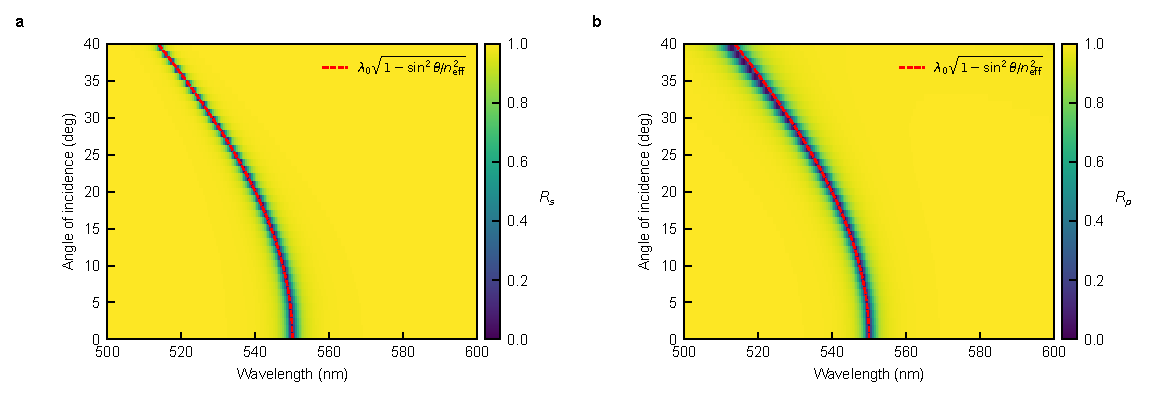
\includegraphics[width=\textwidth]{11_angle_wavelength_map.pdf}
  \caption{Two-dimensional reflectance map $R(\theta_0, \lambda)$ of the bandpass filter for $s$ (a) and $p$ (b) polarisation. The dark vertical streak is the narrow cavity resonance, seen here as a dip in reflectance; the dashed red curve is the analytic passband shift of equation~\eqref{eq:map-shift} with $n_{\rm eff} = \sqrt{n_H n_L}$.}
  \label{fig:map}
\end{figure}

The analytic curve tracks the minimum of $R(\theta_0, \lambda)$ in both
maps without adjustable parameters, which validates the angular dispersion
of the stack up to the approximation used in $n_{\rm eff}$. A second
feature emerges at oblique incidence: the $s$ and $p$ maps are no longer
identical. The $p$ map shows a shallower and slightly broader dip at large
$\theta_0$ because each interface carries a different Fresnel coefficient
for $p$ polarisation, which reduces the effective mirror reflectance and
broadens the cavity line. This polarisation splitting of the passband is
the exact quantity that tilted-incidence bandpass filters are designed
around, and it is reproduced here from first principles without any
effective-medium fit parameter.


